%% DPN-Bench -- IEEE conference format (IEEEtran)
%% Compile: pdflatex dpn_bench_ieee.tex  (twice, + bibtex if you switch to .bib)
\documentclass[conference]{IEEEtran}
\IEEEoverridecommandlockouts
\usepackage{cite,amsmath,amssymb,graphicx,booktabs,url,multirow}
\usepackage[hidelinks]{hyperref}
\def\BibTeX{{\rm B\kern-.05em{\sc i\kern-.025em b}\kern-.08em T\kern-.1667em\lower.7ex\hbox{E}\kern-.125emX}}

\begin{document}

\title{DPN-Bench: A Mechanism-Anchored Multi-Task Benchmark and\\
Audited Virtual Screen for Painful Diabetic Neuropathy}

\author{\IEEEauthorblockN{[Author]}
\IEEEauthorblockA{[Affiliation]\\
[email]}}

\maketitle

\begin{abstract}
Painful diabetic peripheral neuropathy (DPNP) affects a large fraction of the
diabetic population, and its four guideline first-line drugs---duloxetine,
pregabalin, gabapentin and amitriptyline---produce clinically meaningful relief
in only about 40\,\% of patients. Computational screening could widen the
candidate pool, but existing molecular machine-learning benchmarks are organised
by convenience rather than by disease mechanism, and published virtual screens
of phytochemicals rarely audit their own hits for assay-interference artefacts.
We assemble \textbf{DPN-Bench}, a 15-task benchmark of PubChem high-throughput
endpoints selected for mechanistic linkage to DPNP, spanning an analgesic
ion-channel arm (TRPV1, Kv7.2/KCNQ2, two-pore K$^+$), matched pro-excitatory
counter-screens, and a neuroprotective arm (Nrf2/ARE, CHOP, unfolded-protein
response, STEP). After curation the benchmark contains 415{,}085 molecules over
104{,}706 Bemis--Murcko scaffolds at 0.01--3.8\,\% positive rate, evaluated under
a scaffold split with 1.85\,\% train/test scaffold leakage. A multi-task
feed-forward network over ECFP4 and physico-chemical descriptors reaches a mean
ROC-AUC of 0.824, BEDROC($\alpha{=}80.5$) of 0.260 and 1\,\% enrichment factor of
22.0, outperforming LightGBM (0.788 / 0.232 / 18.8), logistic regression and a
Tanimoto similarity-search control, and winning 9 of 15 tasks on BEDROC. We then
screen 59 guideline drugs, aldose-reductase inhibitors, phytochemicals and
negative controls, reporting conformal $p$-values and applicability-domain
distances alongside every score. An interference audit changes the conclusion
materially: 11 of 59 library compounds carry PAINS alerts, three are memorised
training actives, and $\alpha$-tocopherol reaches the top 5\,\% of seven
unrelated tasks. We further show the model systematically misses covalent
Nrf2 activators (sulforaphane 32nd percentile, $\alpha$-lipoic acid 28th)
despite their strong clinical rationale. We argue that reporting this audit is a
necessary component of any phytochemical virtual screen, and release the full
pipeline, which trains on a single CPU core with no deep-learning dependency.
\end{abstract}

\begin{IEEEkeywords}
diabetic neuropathy, neuropathic pain, virtual screening, multi-task learning,
conformal prediction, PAINS, drug repurposing, cheminformatics
\end{IEEEkeywords}

\section{Introduction}

Diabetic peripheral neuropathy occurs in up to half of patients with diabetes
mellitus. Current pharmacotherapy is symptomatic: all major guidelines recommend
a gabapentinoid, a tricyclic antidepressant or an SNRI first line, and the
OPTION-DM crossover trial found amitriptyline, duloxetine and pregabalin
comparably effective, with combination therapy helping patients who fail
maximum-tolerated monotherapy~\cite{optiondm}. None of these agents restores
nerve function, and only pregabalin and duloxetine hold a regulatory indication.
This leaves a genuine therapeutic gap and an obvious role for computational
candidate generation.

Two problems limit the usefulness of existing work. First, molecular
machine-learning benchmarks (MoleculeNet, and the disease-tagged MolData
collection~\cite{moldata}) are organised around data availability, so a model
that performs well on them has not been shown to perform well on the targets
that matter for a given indication. Second, the large literature applying
machine learning to herbal and phytochemical libraries overwhelmingly reports
top-ranked hits without auditing them: polyphenols such as quercetin, luteolin
and epigallocatechin gallate are notorious high-throughput-screening frequent
hitters and carry PAINS substructure alerts~\cite{pains,baell}, yet they recur as
``predicted actives'' across unrelated targets.

\textbf{Contributions.}
\begin{enumerate}
\item \textbf{DPN-Bench}, a 15-task benchmark whose endpoints are selected for
mechanistic linkage to DPNP rather than for data volume, with a documented
scaffold split and leakage measurement.
\item A multi-task network that outperforms gradient boosting, a linear model
and a similarity-search control on the panel, implemented in NumPy so the
benchmark is reproducible without a GPU.
\item An \textbf{audited} virtual screen in which every score is accompanied by a
conformal $p$-value, an applicability-domain distance, a PAINS flag and a
promiscuity count --- and in which the audit demonstrably overturns the naive
ranking.
\item A negative result we consider the most useful part of the paper: the model
fails on precisely the covalent Nrf2 activators ($\alpha$-lipoic acid,
sulforaphane) with the strongest DPN clinical rationale, for reasons intrinsic
to fingerprint representations.
\end{enumerate}

\section{Related Work}

\textbf{Benchmarks.} MolData~\cite{moldata} assembled roughly 170 million
screening results over 1.4 million molecules from PubChem, tagged by disease and
target category, with scaffold splits. We use it as our substrate but re-select
endpoints by mechanism.

\textbf{Graph and foundation models.} TxGNN~\cite{txgnn} formulates repurposing
as zero-shot link prediction over a 17{,}080-disease knowledge graph and improves
indication accuracy by 49.2\,\% over eight baselines; it is complementary to our
ligand-centric setting. Boltz-2~\cite{boltz2} is the first model to approach
free-energy-perturbation accuracy for binding affinity, but an independent
evaluation reports a ``regression to the centre'' effect, with most predictions
compressed into $-5$ to $-8$\,kcal/mol and no meaningful correlation with
physics-based calculations among its own top-ranked
compounds~\cite{boltzreliability}. We therefore treat structure-based affinity
prediction as out of scope and benchmark ligand-based models honestly instead.

\textbf{Early-recognition metrics.} ROC-AUC is near-useless at 0.3\,\%
prevalence because it integrates over regions no screener inspects. We report
BEDROC~\cite{bedroc} and enrichment factors as primary.

\section{DPN-Bench Construction}

\subsection{Mechanistic endpoint selection}
Table~\ref{tab:panel} lists the panel. Each arm is tied to an agent with
clinical standing in DPNP: the capsaicin 8\,\% patch is approved for DPNP of the
feet (TRPV1 agonism); retigabine and flupirtine are Kv7/KCNQ openers; TREK-1
(two-pore K$^+$) activation is analgesic; and the neuroprotective arm targets the
oxidative- and ER-stress axes that dominate DPN pathogenesis and that constitute
the shared mechanism of $\alpha$-lipoic acid, curcumin and sulforaphane.
Pro-excitatory directions (KCNQ2 block, K2P block) are retained deliberately as
\emph{counter-screens}: a candidate scoring highly on both the opener and the
blocker task is not selective.

\begin{table}[t]
\caption{The DPN-Bench panel. $n_{+}$ = test-split positives.}
\label{tab:panel}
\centering\footnotesize
\begin{tabular}{@{}llrr@{}}
\toprule
Arm & Task (PubChem AID) & $n$ test & $n_{+}$ \\
\midrule
\multirow{4}{*}{Analgesic}
 & TRPV1 agonist (540275)        & 28{,}951 & 46 \\
 & KCNQ2 potentiator (2239)      & 30{,}254 & 183 \\
 & K2P activator (623877)        & 32{,}958 & 124 \\
 & TRP agonist (1424)            & 27{,}419 & 44 \\
\midrule
\multirow{3}{*}{Counter-screen}
 & KCNQ2 inhibitor (2156)        & 30{,}258 & 402 \\
 & K2P inhibitor (602410)        & 33{,}880 & 336 \\
 & K2P inhibitor 2 (488922)      & 30{,}258 & 417 \\
\midrule
\multirow{6}{*}{Neuroprotective}
 & Nrf2/ARE activator (624171)   & 36{,}722 & 144 \\
 & CHOP inhibitor (2732)         & 27{,}463 & 976 \\
 & UPR apoptotic (449763)        & 32{,}096 & 158 \\
 & UPR adaptive (463104)         & 32{,}096 & 149 \\
 & STEP inhibitor (588621)       & 36{,}825 & 105 \\
 & $\beta$-cell protection (435005) & 29{,}727 & 324 \\
\midrule
\multirow{2}{*}{Auxiliary}
 & HKDC1 inhibitor (493160)      & 34{,}098 & 98 \\
 & HKDC1 activator (493187)      & 34{,}098 & 40 \\
\bottomrule
\end{tabular}
\end{table}

\subsection{Curation and split}
From MolData we stream the 18 panel columns, retaining molecules with at least
one non-missing label (416{,}909). We desalt to the largest organic fragment,
strip isotopes, sanitise, restrict to 6--70 heavy atoms, and deduplicate on
canonical SMILES merging labels by maximum. This yields \textbf{415{,}085}
molecules over \textbf{104{,}706} Bemis--Murcko scaffolds. We adopt MolData's
official scaffold split (347{,}197 / 28{,}379 / 39{,}509) and \emph{measure}
rather than assume its difficulty: only 1.85\,\% of test scaffolds also appear in
training. Three endpoints with fewer than 40 test positives are trained as
auxiliary heads but excluded from evaluation.

Features are ECFP4 (Morgan radius 2, 1024 bits, stored sparse) concatenated with
14 fast physico-chemical descriptors, $z$-scored using training statistics only.

\section{Models}

\textbf{MTL-FCNN.} A shared trunk $1038 \to 512 \to 128$ with ReLU and inverted
dropout ($p{=}0.25$), and 18 sigmoid heads. The loss is a masked, positive-weighted
binary cross-entropy,
\begin{equation}
\mathcal{L} = \frac{\sum_{i,j} m_{ij}\,w_j^{y_{ij}}\,\ell(z_{ij},y_{ij})}
                   {\sum_{i,j} m_{ij}\,w_j^{y_{ij}}},
\end{equation}
where $m_{ij}=1$ iff assay $j$ tested molecule $i$, and $w_j$ is the clipped
negative/positive ratio for task $j$. Masking is what makes multi-task learning
legitimate here: PubChem assays test overlapping but non-identical decks, so a
molecule contributes gradient only to heads that actually measured it.
Optimisation is Adam ($\eta{=}10^{-3}$, batch 512). The implementation is plain
NumPy; a float64 central-difference gradient check reports a worst relative
error of $2.3\times10^{-6}$, the truncation floor for $\epsilon{=}10^{-3}$.
Training converges by epoch 13 at 12\,s/epoch on one CPU core.

\textbf{Baselines.} (i) LightGBM per task on ECFP4; (ii) $\ell_2$ logistic
regression; (iii) a \emph{Tanimoto $k$-NN similarity-search control} scoring each
test molecule by mean Tanimoto to its five nearest training actives. The third
is essential: a QSAR model that cannot beat ``retrieve the most similar known
active'' has learned nothing beyond lookup.

\textbf{A note on negative subsampling.} Retaining 40k negatives per task rather
than all ${\sim}300$k made LightGBM both ${\sim}8\times$ faster and
\emph{better} (Nrf2: ROC-AUC 0.867 vs 0.796; EF1\,\% 27.8 vs 19.5). The
full-data configuration was degraded by early stopping on a validation metric
that is unstable at 0.3\,\% prevalence. We report this because it is a trap
rather than a trick.

\section{Benchmark Results}

\begin{table}[t]
\caption{Held-out test performance, mean over the 15 evaluated tasks.}
\label{tab:main}
\centering\footnotesize
\begin{tabular}{@{}lcccc@{}}
\toprule
Model & ROC-AUC & $\Delta$PR-AUC & BEDROC & EF 1\,\% \\
\midrule
Tanimoto $k$-NN      & 0.663 & 0.043 & 0.174 & 14.4 \\
Logistic regression  & 0.771 & 0.030 & 0.144 & 11.6 \\
LightGBM             & 0.788 & 0.075 & 0.232 & 18.8 \\
\textbf{MTL-FCNN}    & \textbf{0.824} & \textbf{0.075} & \textbf{0.260} & \textbf{22.0} \\
\bottomrule
\end{tabular}
\end{table}

\begin{figure}[t]
\centering
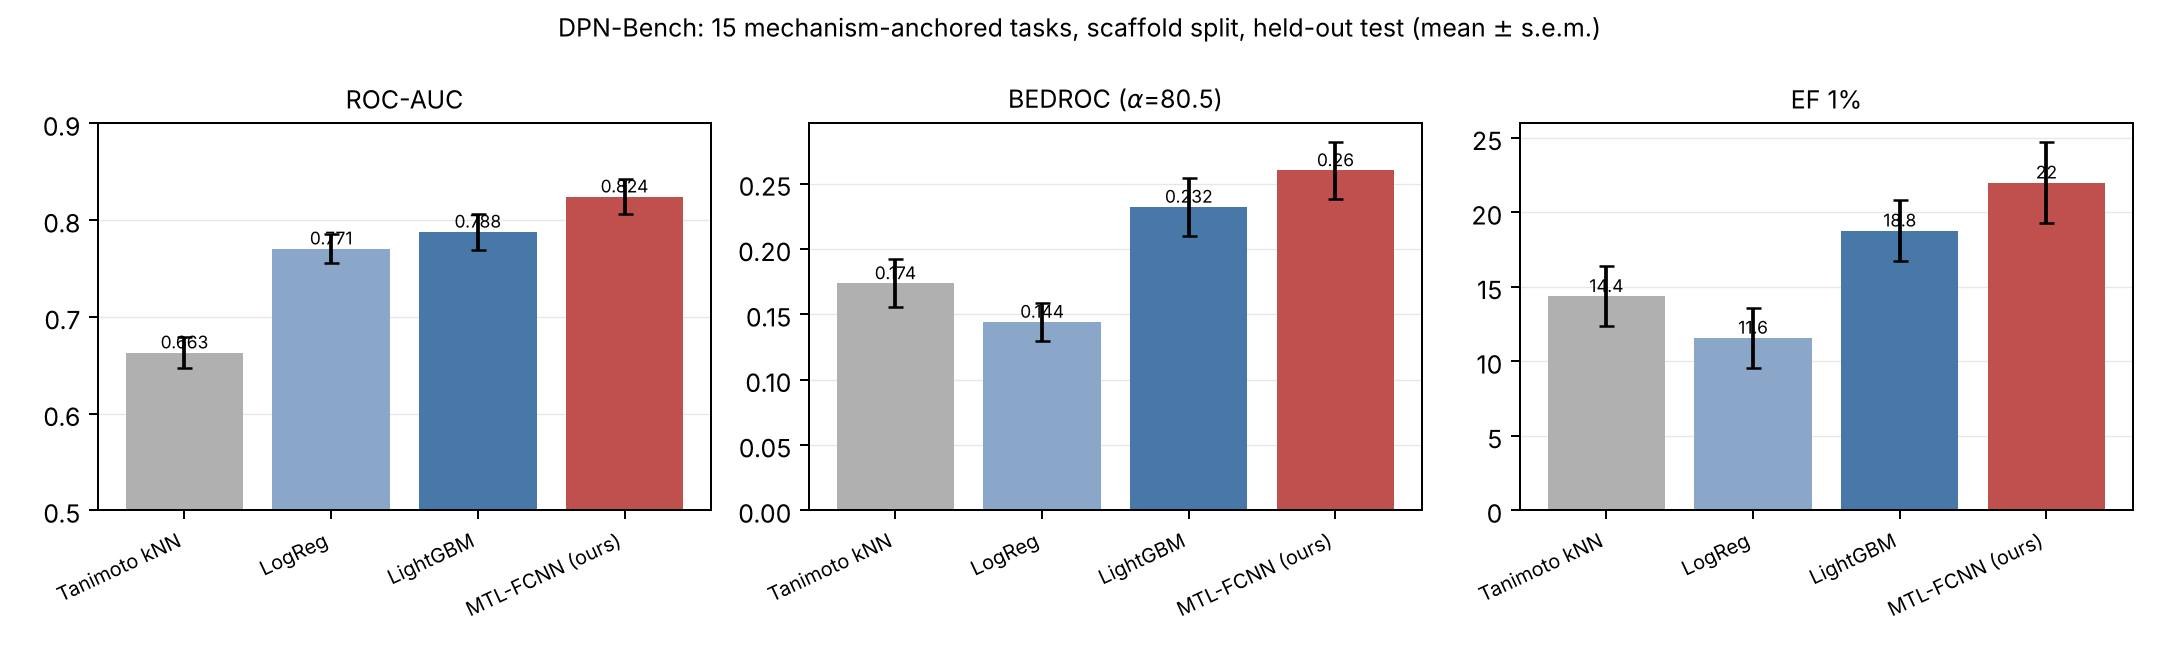
\includegraphics[width=\columnwidth]{../results/fig_benchmark.png}
\caption{Panel-mean performance ($\pm$ s.e.m. over 15 tasks).}
\label{fig:bench}
\end{figure}

Table~\ref{tab:main} and Fig.~\ref{fig:bench} summarise. MTL-FCNN leads on every
metric and wins 9 of 15 tasks on BEDROC against LightGBM's 6. Two observations
deserve emphasis. First, \textbf{similarity search outperforms the linear model on
early recognition} (BEDROC 0.174 vs 0.144; EF1\,\% 14.4 vs 11.6) while losing
badly on global ROC-AUC --- a reminder that AUC and screening utility diverge at
low prevalence. Second, performance is strongly task-dependent: the K2P activator
endpoint remains near chance (ROC-AUC 0.568), consistent with cell-based
phenotypic read-outs resisting fingerprint QSAR.

\section{Audited Virtual Screen}

We score 59 compounds: guideline first-line agents, adjuncts, six
aldose-reductase inhibitors (the polyol-pathway class, including epalrestat),
phytochemicals with DPN literature, and five negative controls. Each score is
reported with (i) its percentile within the 39{,}509-molecule test deck, (ii) a
Mondrian inductive-conformal $p$-value against validation actives,
$p = (|\{s_i \le s\}|+1)/(n+1)$, and (iii) the maximum Tanimoto to any training
active for that task.

\subsection{Controls}
Negative controls behave: sucrose reaches the 0.4th percentile on KCNQ2
potentiation and glucose the 1.1st on TRPV1 agonism. Retigabine (85.6th
percentile, $T_c{=}0.40$) and flupirtine (63.6th, $T_c{=}0.38$) are recovered as
Kv7 openers by genuine extrapolation, and cinnamaldehyde tops the Nrf2 task
(100th percentile, $T_c{=}0.39$), consistent with its known Michael-acceptor
mechanism. Capsaicin's 99.7th percentile on TRPV1 is \emph{not} a prediction:
$T_c{=}1.00$ shows it is itself a training active.

\subsection{The informative failures}
Sulforaphane (32.3rd percentile, $p{=}0.034$) and $\alpha$-lipoic acid (28.0th,
$p{=}0.026$) --- the two phytochemicals with the strongest DPN rationale, the
latter supported by meta-analyses of symptom scores --- are \emph{missed}. Both
are small electrophiles that activate Nrf2 by covalent modification of KEAP1
cysteines, and both sit far outside the applicability domain
($T_c{=}0.14$--$0.18$). A topological-fingerprint classifier trained on a
reporter-gene assay has no representational capacity for covalent reactivity.
Urea, a negative control, reaches the 65th percentile on the same task,
confirming that the descriptor block misleads on very small molecules. These are
limits of the representation, not of training.

\subsection{Interference audit}
In the unaudited ranking, quercetin, luteolin, mangiferin, EGCG,
ursolic/oleanolic acid and $\alpha$-tocopherol occupied the top positions of
nearly every task. Audit (Table~\ref{tab:audit}) shows why this must be
discarded: 11 of 59 compounds carry PAINS alerts, predominantly the
\texttt{catechol\_A} class; three are memorised training actives; and
$\alpha$-tocopherol enters the top 5\,\% of 7 of 15 mechanistically unrelated
tasks. Removing memorised, PAINS-flagged and promiscuous ($\ge 40\,\%$ of tasks)
compounds and re-ranking yields a materially different and far more sober list,
on which curcumin recurs across the neuroprotective arm at moderate
applicability-domain distance ($T_c \approx 0.4$--$0.6$) and duloxetine scores on
several ion-channel endpoints, consistent with its documented channel
off-targets. Residual false positives persist --- sucrose still reaches the 99th
percentile on K2P activation --- so even the audited list is a hypothesis
generator, not a shortlist.

\begin{table}[t]
\caption{Interference audit of the 59-compound library.}
\label{tab:audit}
\centering\footnotesize
\begin{tabular}{@{}lr@{}}
\toprule
Finding & Count \\
\midrule
Compounds carrying a PAINS alert & 11 / 59 \\
\quad of which \texttt{catechol\_A} & 6 \\
Memorised (is a training active, $T_c \ge 0.99$) & 3 \\
Top 5\,\% on $\ge 40\,\%$ of tasks (promiscuous) & 4 \\
Excluded from audited ranking (union) & 14 \\
\bottomrule
\end{tabular}
\end{table}

\section{Limitations}
Labels are single-concentration primary HTS without dose-response confirmation.
Pathway endpoints (Nrf2, UPR, CHOP) are reporter read-outs, so an ``active'' need
not be a direct binder. Representations are 2D only --- no conformers, docking or
structure. Covalent and redox mechanisms are systematically missed. No ADMET,
blood--nerve-barrier or selectivity modelling is performed, and nothing reported
here has been tested in a cell or an animal. Clinically, duloxetine, pregabalin,
gabapentin and amitriptyline remain the evidence-based first-line agents; this
work does not challenge that.

\section{Conclusion}
Selecting benchmark endpoints by disease mechanism rather than data volume gives
a target panel on which model comparisons are interpretable for a specific
indication, and multi-task learning over such a panel outperforms strong
single-task baselines. More importantly, we show that an interference audit is
not optional hygiene but a result-changing step: without it, our own screen would
have reported a list of PAINS-flagged polyphenols as novel DPNP candidates, which
is approximately what much of the phytochemical virtual-screening literature does
report. We release code, curated data indices and audit tooling so that the audit
can be applied to other screens.

\section*{Reproducibility}
Code, configs, trained weights, benchmark tables and audit outputs:
\url{https://github.com/<user>/dpn-bench}. The pipeline runs on one CPU core
with no deep-learning dependency; \texttt{04\_mtl.py --check} verifies gradients
before training.

\begin{thebibliography}{00}
\bibitem{optiondm} S. Tesfaye \textit{et al.}, ``Comparison of amitriptyline supplemented with pregabalin, pregabalin supplemented with amitriptyline, and duloxetine supplemented with pregabalin for the treatment of diabetic peripheral neuropathic pain (OPTION-DM): a multicentre, double-blind, randomised crossover trial,'' \textit{The Lancet}, vol. 400, no. 10353, pp. 680--690, 2022.
\bibitem{moldata} A. Keshavarzi Arshadi \textit{et al.}, ``MolData: a molecular benchmark for disease and target based machine learning,'' \textit{J. Cheminformatics}, vol. 14, art. 10, 2022.
\bibitem{txgnn} K. Huang, P. Chandak \textit{et al.}, ``A foundation model for clinician-centered drug repurposing,'' \textit{Nature Medicine}, vol. 30, 2024.
\bibitem{boltz2} S. Passaro \textit{et al.}, ``Boltz-2: towards accurate and efficient binding affinity prediction,'' preprint, 2025.
\bibitem{boltzreliability} S. Wan, X. Zhang, X. Xue, P. V. Coveney \textit{et al.}, ``On the reliability of AI methods in drug discovery: evaluation of Boltz-2 for structure and binding affinity prediction,'' arXiv:2603.05532, 2026.
\bibitem{bedroc} J.-F. Truchon and C. I. Bayly, ``Evaluating virtual screening methods: good and bad metrics for the early recognition problem,'' \textit{J. Chem. Inf. Model.}, vol. 47, no. 2, pp. 488--508, 2007.
\bibitem{pains} J. B. Baell and G. A. Holloway, ``New substructure filters for removal of pan assay interference compounds (PAINS) from screening libraries,'' \textit{J. Med. Chem.}, vol. 53, no. 7, pp. 2719--2740, 2010.
\bibitem{baell} J. B. Baell and M. A. Walters, ``Chemistry: chemical con artists foil drug discovery,'' \textit{Nature}, vol. 513, pp. 481--483, 2014.
\bibitem{conformal} V. Vovk, A. Gammerman, and G. Shafer, \textit{Algorithmic Learning in a Random World}. Springer, 2005.
\bibitem{rdkit} G. Landrum \textit{et al.}, ``RDKit: open-source cheminformatics,'' \url{https://www.rdkit.org}.
\end{thebibliography}

\end{document}
